\section{Experimental Evaluation}\label{sec:evaluation}
The method in Section~\ref{sec:methods} is evaluated with a whole-month holdout that approximates the future-oriented test setting.  We report historical and strict protocols separately because their cleaning order and validation rows differ.

\subsection{Protocol and Reproducibility}
The historical protocol follows the recorded BERT pipeline: the full labeled file is cleaned before the time split.  The first 39 months, 2021-01--2024-03, form training; the last 12 months, 2024-04--2025-03, form validation.  The selection run contains 114,627 training rows and 35,058 retained validation rows.  The original validation window has 35,158 rows, of which 100 are removed by full-file rent cleaning.  The four new baseline runs use this same order and score preserved original rents on the retained rows; the saved BERT summary supplies the fifth result.
% Source: ../../results/split.json; ../../results/baselines/round_a/README.md; ../../results/baselines/round_a/scores.csv; ../../results/validation_summary.json.

The strict protocol splits by month first.  It cleans and smooths only training-period rents and fits scaling statistics and the flat-model vocabulary on that period.  HDB vocabularies still come from the auxiliary block table.  Validation passes through the frozen preprocessing state without labels, retaining all 35,158 rows for scoring against original rents.  Only the four baselines have strict results; BERT has not been retrained under this protocol.
% Source: ../../src/scripts/run_baselines.py (prepare); ../../src/preprocess/stage3_encode.py (vocabularies); ../../results/baselines/round_a/README.md; ../../results/baselines/round_a/scores.csv.

RMSE is computed on the SGD/month scale with one equal weight per row; MAE and mean error (prediction minus target) are reported as diagnostics.  The recorded BERT run used seed 42, deterministic float32 settings, Python 3.12.14, PyTorch 2.10.0+cu128, Transformers 4.57.6, NumPy 2.3.5, pandas 3.0.1 and an NVIDIA GeForce RTX 5090 Laptop GPU.  Its refit uses all 149,685 retained training rows, with 40 pretraining epochs and 7 fine-tuning epochs selected in the preceding round.  Code, configurations and recorded summaries are available in the project repository.\footnote{\url{https://github.com/MOYU114/cs-5228-proj}. Reproduction commands and environment requirements are in the project and baseline READMEs. Raw course data, checkpoints and BERT row-level predictions are external to Git.}
% Source: ../../results/split.json; ../../results/environment.json; ../../results/refit.json; ../../src/bert_rent/run.py; ../../README.md, Section 6; ../../results/baselines/round_a/README.md. Repository URL verified from git remote origin.

\subsection{Model Comparison (RQ1)}
Table~\ref{tab:model_comparison} compares models under the historical protocol.  The recent grouped mean already reduces RMSE from 842.54 to 497.97 SGD/month, indicating that a large part of the predictable variation is captured by recent town--flat-type price levels.  Shallow CatBoost and the two-stage BERT are nearly tied in RMSE: their difference is 0.23 SGD/month.  BERT has lower MAE and a smaller absolute bias.  These are descriptive results from a single historical window, not evidence of a statistically established or general model ranking.  The best RMSE improves on the recent grouped mean by only about 30 SGD/month.

\begin{table}[t]
\caption{Historical-protocol model comparison on 35,058 retained validation rows.  Bias is prediction minus the original recorded rent; all metrics are SGD/month.}
\label{tab:model_comparison}
\centering
\footnotesize
\begin{tabularx}{\columnwidth}{@{}Xrrr@{}}
\toprule
Model & RMSE & MAE & Bias \\
\midrule
Global mean & 842.54 & 686.73 & $-534.45$ \\
Recent 6-month town$\times$flat-type mean & 497.97 & 374.20 & $-51.09$ \\
Ridge & 606.82 & 459.95 & $+371.92$ \\
Shallow CatBoost & 468.11 & 348.07 & $-37.46$ \\
Two-stage BERT & 468.34 & 344.83 & $-6.73$ \\
\bottomrule
\end{tabularx}
\end{table}
% Source: ../../results/baselines/round_a/scores.csv (historical rows); ../../results/validation_summary.json (two-stage BERT original-label row). About 30 SGD = 497.9674502819732 - 468.11344433391184.

The project README records 86.2 million regression-model parameters and about 4~h~45~min for BERT selection plus refitting on a GPU.  The historical CatBoost fit-and-predict pass took about 9~s on a CPU, excluding preprocessing.  The different hardware and timing scopes preclude a controlled speed comparison.
% Source: ../../README.md, Sections 3 and 5 (recorded parameter count and training times); ../../results/baselines/round_a/scores.csv (fit_predict_seconds); ../../results/baselines/round_a/README.md.


\subsection{Feature-Group Ablation (RQ2)}
Table~\ref{tab:ablation} reports strict-protocol ablations, each retraining the same model and configuration after removing one group.  Removing street and building IDs raises RMSE by 8.52 for Ridge and 2.95 for CatBoost.  Removing ten facility fields changes RMSE by less than 1 SGD/month with town, coordinates and other location fields retained.  The largest increases follow removal of the time group: +85.64 for Ridge and +232.26 for CatBoost.  Because all other groups stay in the model, each $\Delta$ measures a group's additional predictive value given the remaining features, not its standalone importance.
% Source: ../../results/baselines/round_a/ablation.csv; ../../src/scripts/run_baselines.py (ABLATIONS).

The time group contains five fields: month index, two cyclic components, lease-based age and completion age.  Its joint effect cannot be assigned to any single field.  CatBoost's strict bias shifts from $-33.28$ to $-505.62$ SGD/month without this group, approaching the strict global-mean bias of $-528.94$.  This is consistent with losing the ability to track the later rental level, even though time-filtered MRT features can still carry indirect time information.  BERT has no feature-group ablation.
% Source: ../../results/baselines/round_a/scores.csv (strict B3_catboost/full, B3_catboost/no_explicit_time, B0_mean/full); ../../results/baselines/round_a/README.md. Interpretation of bias is an inference from these results.

\begin{table}[t]
\caption{Strict-protocol ablation on all 35,158 validation rows (SGD/month). First row: full-input RMSE; remaining rows: $\Delta$RMSE. Deltas are computed before rounding.}
\label{tab:ablation}
\centering
\footnotesize
\begin{tabularx}{\columnwidth}{@{}Xrr@{}}
\toprule
Input / removed group & Ridge & CatBoost \\
\midrule
Complete input (RMSE) & 615.49 & 475.83 \\
\midrule
Street and building IDs ($\Delta$RMSE) & $+8.52$ & $+2.95$ \\
Ten facility fields ($\Delta$RMSE) & $-0.08$ & $+0.84$ \\
Time group, five fields ($\Delta$RMSE) & $+85.64$ & $+232.26$ \\
\bottomrule
\end{tabularx}
\end{table}
% Source: ../../results/baselines/round_a/ablation.csv.

\subsection{Target Convention and Within-Input Variation}
For completeness, Table~\ref{tab:validation_results} reports the same BERT predictions under the cleaned and preserved original labels.  The cleaned target is used for early stopping; the original target is closer to the uncleaned competition label.  They are scoring conventions for one historical model, not two methods.

\begin{table}[t]
\caption{Historical BERT selection-round scores under two target conventions.  Both rows use the 35,058 retained validation rows; RMSE and MAE are SGD/month.}
\label{tab:validation_results}
\centering
\footnotesize
\begin{tabular}{@{}lrrrr@{}}
\toprule
Scoring target & $n$ & RMSE & MAE & Mean error \\
\midrule
Cleaned rent & 35,058 & 437.16 & 317.74 & $-6.73$ \\
Original rent & 35,058 & 468.34 & 344.83 & $-6.73$ \\
\bottomrule
\end{tabular}
\end{table}
% Source: ../../results/validation_summary.json.

For a group of identical inputs, every model must emit one value; the group mean is optimal for squared error, while deviations of the recorded rents around that mean remain.  On this retained validation set, the two recorded RMSE values satisfy the decomposition in Eq.~\ref{eq:decomp}:
\begin{equation}
\label{eq:decomp}
468.3424^2 \approx 437.1584^2 + 168.04^2.
\end{equation}
Thus 168.04 SGD is the RMS within-input variation isolated by this decomposition.  It is a data-dependent diagnostic floor for a model restricted to the supplied fields, not proof that every future row has the same irreducible component.
% Source: ../../results/validation_summary.json; ../../src/preprocess/rent_cleaning.py. The 168.04 value is computed from the two recorded RMSE values.

\subsection{Error Analysis (RQ3)}
Figure~\ref{fig:validation_month} shows month-wise BERT error.  The upper panel contains the two RMSE curves; the lower panel shows monthly mean error as bars.  On the original labels, RMSE is high in 2024-04 (503.3 SGD) and 2024-06 (496.6 SGD) and falls below 445 SGD in 2025-02 and 2025-03.  Mean error moves from +32.9 SGD in 2024-06 to $-52.8$ SGD in 2025-03, so the model is initially high and later low relative to the observed labels.  This sign change indicates residual temporal drift.

The baseline files provide complementary temporal evidence.  In the historical window, shallow CatBoost has lower monthly RMSE in the first five months, whereas BERT is lower in the final seven months.  Ridge's historical monthly mean error grows from approximately +218 SGD in 2024-04 to +532 SGD in 2025-03, a pattern consistent with overly strong linear time extrapolation.  Figure~\ref{fig:model_bias} shows these monthly biases.  The recent six-month town--flat-type mean (RMSE 497.97) is also more accurate than Ridge (606.82) in Table~\ref{tab:model_comparison}: even with area and location inputs, how the past rent trend is carried into future months strongly affects the estimate.
% Source: ../../results/baselines/round_a/by_month.csv (historical, full features); ../../results/validation_summary.json (BERT by_month mean_error); ../../results/baselines/round_a/scores.csv. Figure: photo/make_figures.py, model_bias_by_month().

% Source: ../../results/validation_summary.json; ../../results/baselines/round_a/by_month.csv; ../../results/baselines/round_a/README.md.

\begin{figure}[t]
\centering
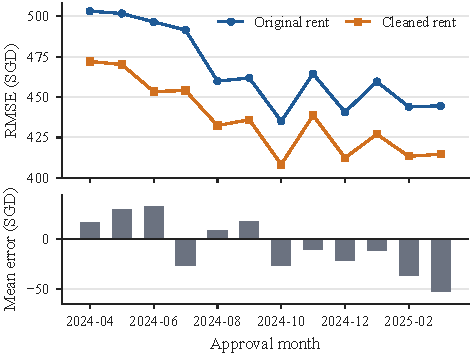
\includegraphics[width=\columnwidth]{fig4_validation_by_month.pdf}
\caption{Historical BERT validation by approval month for the same 35,058 retained rows.  The upper panel shows RMSE on cleaned and original recorded rents; the lower panel shows mean error (prediction minus original recorded rent).  All values are SGD/month.}
\label{fig:validation_month}
\end{figure}

\begin{figure}[t]
\centering
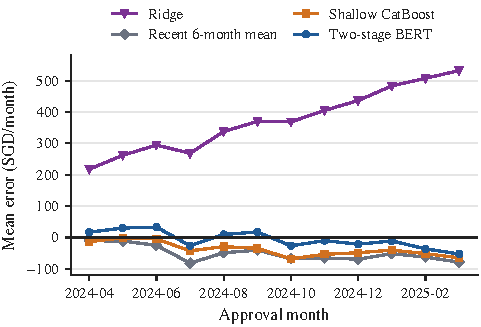
\includegraphics[width=\columnwidth]{fig6_model_bias_by_month.pdf}
\caption{Monthly mean error (prediction minus original recorded rent) under the historical protocol, 35,058 retained validation rows, SGD/month.  Ridge over-predicts increasingly over time, while the other models stay within 85~SGD of zero.  The global mean (bias about $-500$) is omitted for scale.}
\label{fig:model_bias}
\end{figure}

Building coverage exposes a second generalization boundary.  Under the strict protocol, CatBoost RMSE is 475.50 for buildings seen during training and 548.26 for unseen buildings; the unseen group contains only 151 rows.  The small unseen sample makes that estimate uncertain.  BERT's row-level predictions are unavailable for this building-level breakdown.
% Source: ../../results/baselines/round_a/by_building_seen.csv; ../../results/baselines/round_a/README.md.

Figure~\ref{fig:predicted_recorded} compares BERT predictions with recorded rents.  The diagonal trend is captured, while the prediction range is visibly narrower than the observed range, indicating shrinkage toward typical rents for the represented field combinations.  The available fields do not identify the omitted unit attributes behind individual residuals.

\begin{figure}[t]
\centering
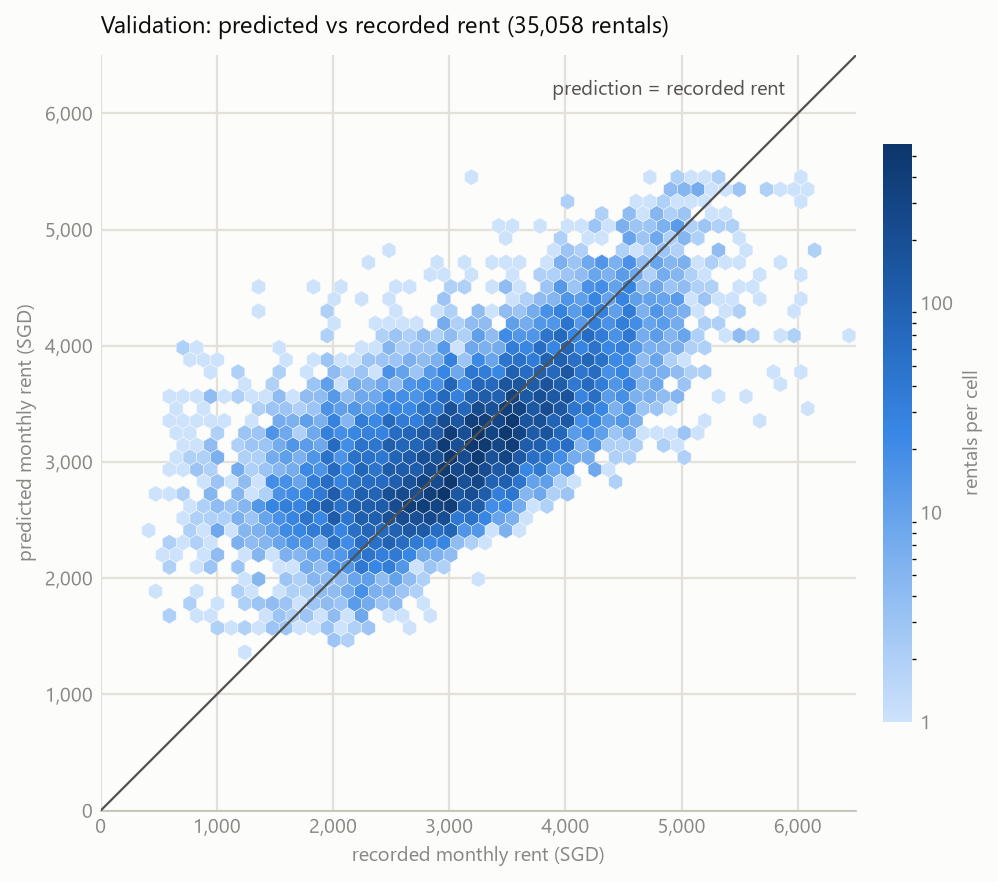
\includegraphics[width=0.92\columnwidth,trim=0 0 0 18bp,clip]{fig5_predicted_vs_recorded.png}
\caption{Predicted versus original recorded validation rent for 35,058 retained rows.  Both axes are SGD/month; the diagonal is the identity line.}
\label{fig:predicted_recorded}
\end{figure}

% Source: ../../results/figures/fig3_predicted_vs_recorded.png; ../../results/validation_summary.json. Legacy PNG retained; LaTeX clips its title only, without new row-level analysis.
